\documentclass[professionalfont, handout, 10pt]{beamer} %, handout



%\usepackage{pxfonts}
%\usepackage{eulervm}

%\documentclass[sans,mathserif]{beamer}
%\usepackage{kerkis} % Kerkis roman and sans
%\usepackage{kmath}


%\documentclass[serif, professionalfont]{beamer} %
%\usepackage[T1]{fontenc} % Needed for Type1 Concrete
%\usepackage{concrete}


\usepackage{amsmath}
\usepackage{amsthm}
\usepackage{amsthm,amssymb,amsfonts,amsmath} 
% \usepackage{proof}
\usepackage[mathscr]{eucal}
\usepackage{amssymb,mathtools}
\usepackage{xcolor}
\usepackage{mathrsfs}
\usepackage{enumerate}

\usepackage{tikz}
\usetikzlibrary{shapes.geometric}
\usetikzlibrary{arrows}
\usetikzlibrary{shapes}
\usetikzlibrary{plotmarks}

 
 

\theoremstyle{plain}
\newtheorem{thm}{Theorem}
\newtheorem{remark}{Remark}
\newtheorem{cor}[thm]{Corollary}
 
\theoremstyle{definition}
\newtheorem{df}{Definition}
       
  
\usepackage{epsfig}
%\usepackage{amsmath}
%\usepackage{mathrsfs}
%\usepackage[all]{xy}  
%\usepackage{proof}    %%proof.style file
           

\newcommand{\tcb}[1]{\textcolor{blue}{#1}}
\newcommand{\tcr}[1]{\textcolor{red}{#1}}  
\newcommand{\tcc}[1]{\textcolor{cyan}{#1}}
\newcommand{\tcg}[1]{\textcolor{green}{#1}} 
\newcommand{\tcm}[1]{\textcolor{magenta}{#1}}      

\newcommand{\omt}{\mathop{\curlywedge}}
  
    
\newcommand{\Lra}{\: \Leftrightarrow \:}
\newcommand{\m}[1]{{\mathbf {#1} }}
%\newcommand{\m}[1]{{\mbox{\uppercase {\bf {#1}}}}}
%\newcommand{\N}[1]{{{ \m N_{#1}}}}
\newcommand{\Rl}{ {\mbox{$\mathcal{RL}  $}}}
\newcommand{\Rlc}{ {\mbox{$\mathcal{RL}^C  $}}}
\newcommand{\Ra}{{ \:\; \Rightarrow \:\; }}
%\newcommand{\Ra}{{\mbox{$ \: \Rightarrow \: $}}}
\newcommand{\Rar}{{ \: \Rightarrow \: }}
\newcommand{\La}{{\mbox{$ \: \Leftarrow \: $}}}
\newcommand{\ra}{\rightarrow}
\newcommand{\la}{\leftarrow}
\newcommand{\lra}{\leftrightarrow}
\newcommand{\fa}{\: \forall}
\newcommand{\lan}{(}
\newcommand{\ran}{)}
\newcommand{\rl}{{residuated lattice }}
\newcommand{\rls}{{residuated lattices }}
\newcommand{\T}{\top}
\newcommand{\jn}{\vee}
\newcommand{\mt}{\wedge}
\newcommand{\ror}{\: $ or $ \:}
\newcommand{\rand}{\: $ and $ \:}
\newcommand{\Tg}{\lan \T \ran}
\newcommand{\set}[2]{{\mbox{$ \{ #1 \: | \: #2 \}  $}}}
\newcommand{\ex}{\exists}
\newcommand{\eq}{\approx}
\newcommand{\eqv}{\cong}
\newcommand{\sbs}{\subseteq}
\newcommand{\sps}{\supseteq}
\newcommand{\vr}{{\mbox{$\mathcal{V}$}}}
\newcommand{\Vr}{{\mbox{$ \mathcal{V} \: $ }}}
\newcommand{\vrg}[1]{{\mbox{ $ \mathcal{V}  (\m #1) $}}}
\newcommand{\vs}{\emptyset}
\newcommand{\cov}{\prec}
\newcommand{\rd}{{/}}
\newcommand{\ld}{{\setminus}}
%\newcommand{\qed}{\hfill$\bullet$}
\newcommand{\ol}{\overline}
%\newcommand{\ua}{\hspace{.04in} \uparrow \hspace{-.04in}}
\newcommand{\ua}{\mathop{\uparrow}}
\newcommand{\da}{\hspace{.01in} \downarrow \hspace{-.01in}}
\newcommand{\dm}{\stackrel{\cdot}{-}}
\newcommand{\md}{\stackrel{-}{\cdot}}
\newcommand{\bra}{{\bf \ra}}
\newcommand{\blra}{{\bf \lra}}
\newcommand{\ban}{{\bf \&}}
\newcommand{\bor}{{\bf \nabla}}
\newcommand{\bmt}{{\bf \mt}}
\newcommand{\bjn}{{\bf \jn}}
\newcommand{\bneg}{{\bf \neg}}
\newcommand{\bbot}{{\bf \bot}}
\newcommand{\btop}{{\bf \top}}
\newcommand{\entails}{\vdash}
\newcommand{\TM}{{\mbox{{Turing Machine }}}}
\newcommand{\TMs}{{Turing Machines }}
\newcommand{\MM}{{Minskii Machine }}
\newcommand{\RA}{\Ra}
\newcommand{\rla}{{relation algebra }}
\newcommand{\rlas}{{relation algebras }}
\newcommand{\cv}{ ^{ \cup } }
\newcommand{\cg}{{\rm Cg}}                          %Petar
\newcommand{\var}[1]{{\uppercase \mathcal{{#1}}}}      %Petar
\newcommand{\Lg}{{\mbox{$\mathcal{LG} $}}}             %Partick
\newcommand{\Lgm}{{\mbox{$\mathcal{LG}^- $}}}          %Partick
\newcommand{\phibar}{{\mbox{$\ol \phi\ $}}}         %Partick
\newcommand{\vrm}{{\mbox{$\mathcal{V}^- $}}}           %Partick
\newcommand{\Ya}{\Rightarrow}
\newcommand{\bs}{\boldsymbol}
\newcommand{\cleq}{\preceq}
\newcommand{\hra}{\rightharpoonup}
\renewcommand{\ln}{\mathord{\sim}}
\newcommand{\rn}{\mathord{-}}
\newcommand{\lrh}{\mathop{\leftrightarrow}}
\providecommand{\semsb}{\ensuremath{\mathscr{M}}}
\providecommand{\sem}[1]{\ensuremath{\semsb (#1)}} 
\newcommand{\alhack}{\\[-\normalbaselineskip]\tag*{\qedhere}}
\providecommand{\psetsb}{\ensuremath{\mathscr{P}}}
\providecommand{\pset}[1]{\ensuremath{\psetsb (#1)}} 
\providecommand{\pfin}[1]{\ensuremath{\psetsb_{\text{fin}}(#1)}}

\newcommand{\co}{\mathsf} %fontshape for class operators
\newcommand{\cl}{\mathcal} %fontshape for general classes
\newcommand{\RL}{\va{RL}}
\DeclareMathOperator{\Mod}{Mod}
\newcommand{\bl}{\boldsymbol{\Lambda}}

% Macros for FL
\newcommand{\al}{\alpha}
\newcommand{\sig}{\Sigma}
\newcommand{\lam}{\Lambda}
\newcommand{\gam}{\Gamma}
\newcommand{\del}{\Delta}
\newcommand{\im}{\rightarrow}
\newcommand{\ya}{\rightarrow}
\newcommand{\naraba}{\rightarrow}
\newcommand{\To}{\vdash}
%\newcommand{\lan}{\left(} %not \la
%\newcommand{\ran}{\right)} %not \ra
%\newcommand{\Ya}{\Rightarrow}
\newcommand{\noi}{\noindent}
%\newcommand{\preast}{{\preceq}^{\ast}}
%\newcommand{\prestar}{{\preceq}^{\star}}
\newcommand{\epsi}{\varepsilon}
\newcommand{\e}{\varepsilon}

\newcommand{\p}{\vskip 12pt}
\newcommand{\q}{\vskip 6pt}


\newcommand{\btl}{\lhd}%{\triangleleft}{\blacktriangleleft}
\newcommand{\btr}{\rhd}%{\triangleright}{\blacktriangleright} 
\newcommand{\eb}[1]{\emph{\textcolor{blue}{#1}}}       
\newcommand{\cb}[1]{\textcolor{blue}{#1}} 
\newcommand{\cred}[1]{\textcolor{red}{#1}}        
\newcommand{\ldd}{\mathbin{\bbslash}}
\newcommand{\rdd}{\mathbin{\sslash}}  
\newcommand{\raa}{\mathbin{\leadsto}}    
\newcommand{\RarN}{{\sqsubseteq}}  %{{\mathrel{N}}} 
\newcommand{\RaN}{\mathnormal{\RarN}}

\newcommand{\va}{\mathsf} %fontshape for specific varieties  
\newcommand{\cnv}{u}

\renewcommand{\And}{\text{ \sf and }} %already exists in LaTeX
\newcommand{\Or}{\text{ \sf or }}
\newcommand{\AND}{\text{\sf{AND }}}
\newcommand{\bcdw}{\mbox{\boldmath{$\,\cdot\,$}}}


\renewcommand{\and}{\text{ \sf and }}
\newcommand{\orc}{\text{ \sf or }}
\newcommand{\orb}{\ \overline{\mbox{\sf or}}\ }
\newcommand{\Implies}{\Longrightarrow}
\providecommand{\undsc}{\underline{\phantom{x}}}

\newcommand{\gal}[1]{#1^+}

\newcommand{\force}{\vdash}
\def\hh{\ |\ }
\newcommand{\FL}{\mbox{$\mbox{\bf FL}$}}

\newcommand{\ls}{\setbox0\hbox{$-$}
\mathbin{\hbox{$-$\kern-\wd0\raise2\dp0\hbox{$\cdot$}\kern.3\wd0\lower2\dp0\hbox
{$\cdot$}}}}
\newcommand{\rs}{\setbox0\hbox{$-$}
\mathbin{\hbox{$-$\kern-\wd0\lower2\dp0\hbox{$\cdot$}\kern.3\wd0\raise2\dp0\hbox
{$\cdot$}}}}

\newcommand{\rdo}{\mathop{\mbox{$\bigcirc \! \! \! \! \! \rdd \, $}}}
\newcommand{\ldo}{\mathop{\mbox{$\bigcirc \! \! \! \! \! \ldd \, $}}}

%Lattices 
\providecommand{\MEET}{\ensuremath{\bigwedge}}
\providecommand{\Meet}{\ensuremath{\textstyle\bigwedge\limits}}
\providecommand{\Join}{\ensuremath{\bigvee}}
\providecommand{\meet}{\ensuremath{\wedge}}
\providecommand{\join}{\ensuremath{\vee}}

%Set Theory
\providecommand{\card}[1]{\ensuremath{\left\lvert#1\right\rvert}}
\providecommand{\intersect}{\ensuremath{\cap}}
\providecommand{\Intersect}{\ensuremath{\bigcap}}
\providecommand{\union}{\ensuremath{\cup}}
\providecommand{\UNION}{\ensuremath{\bigcup}}
\providecommand{\Union}{\ensuremath{\textstyle\bigcup\limits}}
%Logic
\providecommand{\iff}{\ensuremath{\Leftrightarrow}}
\providecommand{\implies}{\ensuremath{\Rightarrow}}

%Algebra
\providecommand{\normal}{\ensuremath{\unlhd}}
\providecommand{\embed}{\ensuremath{\hookrightarrow}}%inclusion map
\providecommand{\gen}[1]{\ensuremath{\left<#1\right>}}%Group generated by #1
\providecommand{\idx}[2]{\ensuremath{\left[#1:#2\right]}}%index of #2 in #1
\providecommand{\order}[1]{\ensuremath{\left\lvert#1\right\rvert}}

%Commonly used Sets
\providecommand{\C}{\ensuremath{\mathbb{C}}}%complex
\providecommand{\N}{\ensuremath{\mathbb{N}}}%natural
\providecommand{\Q}{\ensuremath{\mathbb{Q}}}%rationals
\providecommand{\R}{\ensuremath{\mathbb{R}}}%reals
\providecommand{\Z}{\ensuremath{\mathbb{Z}}}%integers
\providecommand{\Zpos}{\ensuremath{\mathbb{Z}^{+}}}%positive integers

%functions
\providecommand{\restrictedto}{\ensuremath{\downharpoonright}}

%Analysis and lineal algebra
\providecommand{\norm}[1]{\ensuremath{\left\lVert#1\right\rVert}}
\providecommand{\vect}{\ensuremath{\vec}}

%Miscellaneous
\providecommand{\abs}[1]{\ensuremath{\left\lvert#1\right\rvert}}
\providecommand{\define}{\ensuremath{\stackrel{\text{\tiny def}}{=}}}

%number theory
\providecommand{\floor}[1]{\ensuremath{\left\lfloor#1\right\rfloor}}
\providecommand{\ceil}[1]{\ensuremath{\left\lceil#1\right\rceil}}

%Miscellaneous shortcuts
\providecommand{\lcm}{\ensuremath{\text{lcm}}}%least common multiple
\providecommand{\st}{\ensuremath{\backepsilon}}

%Presentation dependant
\newcommand{\ccdot}{\bullet}

\newcommand\g[1]{g_{\bf{#1}}}
\newcommand\f[1]{f_{\bf{#1}}}
\newcommand{\gb}{\g{B}}
\newcommand{\gc}{\g{C}}
\newcommand{\fb}{\f{B}}
\newcommand{\fc}{\f{C}}


\usefonttheme[onlymath]{serif}
\usetheme{CambridgeUS} % My favorite!
%with an extra region at the top.
\useoutertheme[subsection=false]{miniframes}%smoothbars}
\definecolor{CrimsonRed}{rgb}{.5882,0,.1804} 
\definecolor{Gold}{rgb}{.6588,.6,.4313}
\definecolor{gold}{HTML}{997316}
\definecolor{Tan}{HTML}{BFB254}%{997316}
%\usecolortheme[named=Tan]{structure} %
%\setbeamercovered{invisible}
%\useoutertheme[right, width=1.8cm]{sidebar}
%\useinnertheme{circles}

\setbeamercolor{palette primary}{fg=CrimsonRed, bg=gold!45!white}
\setbeamercolor{palette sidebar primary}{fg=CrimsonRed} %, bg=gold!20!white}
\setbeamercolor{palette sidebar secondary}{fg=CrimsonRed!90!white}%, bg=gold!18!white}
\setbeamercolor{palette secondary}{fg=CrimsonRed, bg=Gold!30!white}
\setbeamercolor{palette tertiary}{fg=white!80!gold, bg=CrimsonRed}
\setbeamercolor{frametitle}{fg=CrimsonRed, bg=gold!05!white}
\setbeamercolor{title}{fg=gold!40!white, bg=CrimsonRed}
\setbeamercolor{item projected}{bg=Gold!70!white}
 \setbeamercolor{itemize item}{bg=Gold!20!white}
\setbeamertemplate{enumerate items}[default]
\setbeamercolor{block title}{fg=CrimsonRed,bg=gold!35!white}
\setbeamercolor{block body}{fg=black,bg=gold!7!white}
\setbeamercolor{local structure}{fg=Tan!50!white!70!black, }
\setbeamercolor{block title example}{bg=gold!30!white, fg=CrimsonRed}
\setbeamercolor{block body example}{bg=gold!07!white}
%\usecolortheme{sidebartab}

% To remove the navigation symbols from 
% the bottom of slides%
\setbeamertemplate{navigation symbols}{} 
%
\usepackage{graphicx}
%\usepackage{bm}         % For typesetting bold math (not \mathbold)%
%\titlegraphic{\includegraphics[height=1cm]{DU}}
%

\setbeamertemplate{caption}[numbered]
\DeclareMathOperator*{\bigor}{OR}
\newcommand{\bb}[1]{\mathbb {#1}}
\usepackage{setspace}

\title[Residuated lattices over $\m M_X$]{Residuated lattices over $\m M_X$}
\author[Xiao Zhuang]{Xiao Zhuang\\
  \small{(joint work with Nick Galatos)} }
\institute[University of Denver]
{University of Denver}
\date{02.28.23}
% \today will show current date. 
% Alternatively, you can specify a date.
% \titlegraphic{\includegraphics[]{}}
%BEAMER HACKS


%Backgroundcolor
%\setbeamercolor{background canvas}{bg=gold!09!white}



\begin{document}


%\begin{frame}[plain]
%\hspace*{1cm}\parbox[t]{\textwidth}{	
%\titlepage
%}
%\end{frame}


\begin{frame}[plain]{}
%\advance\textwidth1.7cm
\hsize\textwidth
\columnwidth\textwidth
\maketitle

\end{frame}

\section{Introduction}

\begin{frame}{Residuated lattices}
    A residuated lattice is an algebra $(R, \wedge, \vee, \cdot, \backslash, /, 1)$ where
    \begin{itemize}
        \item $(R, \wedge, \vee)$ is a lattice;

        \item $(R, \cdot, 1)$ is a monoid;

        \item For all $x, y, z \in R$,
        \begin{equation}\tag{residuation}\label{res.}
            x \cdot y \leq z \text{ iff } y \leq x \backslash z \text{ iff } x \leq z/x
        \end{equation}
    \end{itemize}

\pause

{\setstretch{1.1} When $(R, \cdot, 1)$ is commutative, (\ref{res.}) is reduced as for all $x, y, z \in R$, $x \cdot y \leq z$ iff $x \leq y \rightarrow z$. \pause

If there exists $a \in R$ such that for all $x \in R$, $(a/x) \backslash a = x = a/(x \backslash a)$, then we call $\m R$ is an \emph{involutive} residuated lattice and denote $a/x = -x$ and $x \backslash a = {\sim} x$.
If we define $x+y := {\sim}[(-y) \cdot (-x)]$, which by involution is equivalent to $-[({\sim}y) \cdot ({\sim}x)]$, we can have $x \backslash y = {\sim}x + y$ and $y/x = x + (-y)$, so (\ref{res.}) is equivalent to for all $x, y, z \in R$
$$x \cdot y \leq z \text{ iff } y \leq {\sim} x + z \text{ iff } x \leq z + (-y)$$}

\end{frame}

\begin{frame}

\begin{block}{Remark}
    \begin{itemize}
        \item A lattice-ordered monoid $\mathbf{R}$ is a reduct of a residuated lattice iff multiplication is order-preserving and for all $x, z \in R$, the sets $\{y \in R: \, xy \leq z\}$ and $\{y \in R: \, yx \leq z\}$ have maximum elements.

        \item A complete lattice-ordered monoid $\mathbf{R}$ is a reduct of a residuated lattice iff multiplication distributes over arbitrary joins.
    \end{itemize}    
\end{block}

\end{frame}

\section{Residuated lattices on $M_X$}

\begin{frame}{Residuated lattices on $M_X$}
Given a set $X$, we denote by $\mathbf{M}_X$ the lattice over the set $X\cup \{\bot, \top\}$, where $\top$ is the top element, $\bot$ is the bottom element, and $x\vee y=\top$ and $x \wedge y=\bot$, for distinct $x,y \in X$.

\begin{figure}[h]
\centering
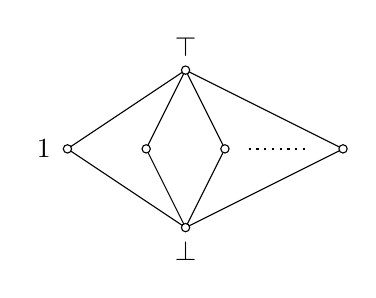
\begin{tikzpicture}
\draw (1.5, 1) -- (0, 0) -- (1.5, -1);
\draw (1.5, 1) -- (1, 0) -- (1.5, -1);
\draw (1.5, 1) -- (2, 0) -- (1.5, -1);
\draw (1.5, 1) -- (3.5, 0) -- (1.5, -1);
\draw[thick, dotted] (2.3, 0) -- (3.05, 0);

\filldraw [color = black, fill = white] (1.5, 1) circle (1.5pt)
(1.5, 1.3) node {$\top$};
\filldraw [color = black, fill = white] (1.5, -1) circle (1.5pt)
(1.5, -1.3) node {$\bot$};
\filldraw [color = black, fill = white] (0, 0) circle (1.5pt)
(-0.3, 0) node {$1$};
\filldraw [color = black, fill = white] (1, 0) circle (1.5pt);
\filldraw [color = black, fill = white] (2, 0) circle (1.5pt);
\filldraw [color = black, fill = white] (3.5, 0) circle (1.5pt);
\end{tikzpicture}
\caption{A residuated lattice over $M_X$}
\end{figure}
\end{frame}

\begin{frame}
    If $X$ is closed under multiplication, then $(X, \cdot, 1)$ is a cancellative monoid. \pause

    A monoid $\mathbf{S}$ with a zero (absorbing element) $0$ is called \emph{$0$-cancellative} if for all $x, y, z \in S$,
    \begin{align*}
        xy = xz \neq 0 & \Rightarrow y = z\\
        yx = zx \neq 0 & \Rightarrow y = z.
    \end{align*}
    
\end{frame}

\begin{frame}{Properties}
In a residuated lattice $\bf{R}$ on $\mathbf{M}_X$, we define
\begin{align*}
    U_R & = \{x \in R \setminus \{\bot, \top\} \, | \, x \top = \top\},\\
    Z_R & = \{x \in R \setminus \{\bot, \top\} \, | \,  x \top = x\}.
\end{align*}

\pause

\begin{itemize}
    \item $\top$ is central in $\mathbf{R}$ and $R = U \sqcup Z \sqcup \{\bot, \top\}$. \pause
    
    \item $U_{\top} = U \cup \{\top\}$ is a $\top$-cancellative submonoid of $\mathbf{R}$. \pause
    
    \item $Z_{\bot} = Z \cup \{\bot\}$ is a subsemigroup of $\mathbf{R}$ with zero $\bot$, $|Z_{\bot}| \leq 3$ and $xy = \bot$ for all distinct $x, y \in Z_{\bot}$.\\    
    Also, either $Z_{\bot}$ is idempotent, or $Z_{\bot} = \{b, \bot\}$ with $b^2=\bot$. \pause
    
    \item $ab = ba = b$ for all $a \in U$ and $b \in Z$.\pause
\end{itemize}

\begin{figure}[h]
\begin{center}
\begin{tabular}{c | c}
 & $\bot$\\
\hline
$\bot$ & $\bot$ 
\end{tabular}
,
\begin{tabular}{c | c c}
 & $\bot$ & $b$\\
\hline
$\bot$ & $\bot$ & $\bot$\\
$b$ & $\bot$ & $b$
\end{tabular}
,
\begin{tabular}{c | c c}
 & $\bot$ & $b$\\
\hline
$\bot$ & $\bot$ & $\bot$\\
$b$ & $\bot$ & $\bot$
\end{tabular}
,
\begin{tabular}{c | c c c}
 & $\bot$ & $b_1$ & $b_2$\\
\hline
$\bot$ & $\bot$ & $\bot$ & $\bot$\\
$b_1$ & $\bot$ & $b_1$ & $\bot$\\
$b_2$ & $\bot$ & $\bot$ & $b_2$ 	
\end{tabular}
\end{center}
\caption{Four multiplication tables of $Z_R$}
\label{f:4tables}
\end{figure}

\end{frame}

\begin{frame}{Construction and Characterization}

$\mathbf{A}$: $\top$-cancellative monoid with zero $\top$ and $\mathbf{B}$: semigroup with zero $\bot$, whose multiplication table is one of those in Figure \ref{f:4tables}.\pause
We define the lattice structure $\mathbf{M}_X$ on the set $R = A \cup B$, where $X = R \setminus \{\bot, \top\}$, $\bot$ is the bottom and $\top$ is the top. \pause
Also, we define a multiplication on $R$ that extends the multiplications on $\mathbf{A}$ and $\mathbf{B}$ by:
\begin{align*}
    xy = yx = y,
\end{align*}
for all $x \in A$ and $y \in B$.
We denote by $\mathbf{R}_{\mathbf{A}, \mathbf{B}}$ the resulting algebra.\pause

\begin{block}{Theorem}
    $\mathbf{R}_{\mathbf{A}, \mathbf{B}}$ is the reduct of a residuated lattice based on $\mathbf{M}_X$, where $X = A \cup B \setminus \{\bot, \top\}$.
\end{block}
\pause

\begin{block}{Corollary}
    The residuated lattices based on $\mathbf{M}_X$ are precisely the ones of the form $\mathbf{R}_{\mathbf{A}, \mathbf{B}}$, where $\mathbf{A}$ is a $\top$-cancellative monoid with zero $\top$ and $\mathbf{B}$ is a semigroup with zero $\bot$, whose multiplication table is one of those in Figure~\ref{f:4tables}.
\end{block}
\end{frame}

\section{Axiomatization}

\begin{frame}{Motivation}

\begin{block}{Facts}
    \begin{itemize}
        \item The multiplicative identity $1$ is an atom on all residuated lattices based on $\mathbf{M_X}$, except for the trivial one and the $3$-element Brouwerian algebra.

        \item The $3$-element Brouwerian algebra is subdirectly irreducible.
    \end{itemize}
\end{block}

\begin{block}{Theorem [Gal+07]}
    Let $\m R$ be a residuated lattice.
    The lattice of convex, normal in $\m R$ submonoid of $R^-$ is isomorphic to the lattice of congruences on $\m R$.
\end{block}

\pause

\begin{block}{Conclusion}
    The residuated lattices based on $\m M_X$ are subdirectly irreducible.
\end{block}
\end{frame}

\begin{frame}{Axiom (URL)}

    A (bounded) residuated lattice is called \emph{unilinear} if it satisfies 
    \begin{equation}\tag{URL}\label{axiom_URL}
        \forall u_1, u_2, z, w \, \, (u_1 \leq u_2 \text{ or } u_2 \leq u_1 \text{ or } (u_1 \wedge u_2 \leq w \text{ and } z \leq u_1 \vee u_2)).
    \end{equation}

    \pause

    \begin{figure}[h]
    \centering
    \begin{tikzpicture}[scale=0.50]
        \draw (3, 4) -- (0, 3);
        \draw[dotted] (0, 3) -- (0, -3);
        \draw (0, -3) -- (3, -4);
        \draw (3, 4) -- (1.5, 3);
        \draw[dotted] (1.5, 3) -- (1.5, -3);
        \draw (1.5, -3) -- (3, -4);
        \draw[dotted] (2, 0) -- (5.5, 0);
        \draw (3, 4) -- (6, 3);
        \draw[dotted] (6, 3) -- (6, -3);
        \draw (6, -3) -- (3, -4);

        \filldraw [color = black, fill = white] (3, 4) circle (2.5pt)
            (3, 4.4) node {$\top$};
        \filldraw [color = black, fill = white] (3, -4) circle (2.5pt)
            (3, -4.4) node [black] {$\bot$};
        \filldraw [color = black, fill = white] (0, 2) circle (2.5pt)
            (-0.3, 2.3) node [black] {};
        \filldraw [color = black, fill = white] (0, 1) circle (2.5pt)
            (-0.3, 1.3) node [black] {};
        \filldraw [color = black, fill = white] (0, 0) circle (2.5pt)
            (-0.3, 0.3) node [black] {};
        \filldraw [color = black, fill = white] (0, -1) circle (2.5pt)
            (-0.4, -0.7) node [black] {};
        \filldraw [color = black, fill = white] (0, -2) circle (2.5pt)
            (-0.4, -1.7) node [black] {};

        \filldraw [color = black, fill = white] (1.5, 2) circle (2.5pt);
        \filldraw [color = black, fill = white] (1.5, 1) circle (2.5pt);
        \filldraw [color = black, fill = white] (1.5, 0) circle (2.5pt)
            (1.2, 0.3) node {};
        \filldraw [color = black, fill = white] (1.5, -1) circle (2.5pt);
        \filldraw [color = black, fill = white] (1.5, -2) circle (2.5pt);

        \filldraw [color = black, fill = white] (6, 2) circle (2.5pt);
        \filldraw [color = black, fill = white] (6, 1) circle (2.5pt);
        \filldraw [color = black, fill = white] (6, 0) circle (2.5pt)
            (6.3, 0.3) node [black] {};
        \filldraw [color = black, fill = white] (6, -1) circle (2.5pt);
        \filldraw [color = black, fill = white] (6, -2) circle (2.5pt);
    \end{tikzpicture}
    \caption{A non-linear unilinear residuated lattice}
    \label{unilinear}
    \end{figure}

\end{frame}

\begin{frame}
\frametitle{Axiom (URL)}
    For these non-linear unilinear residuated lattices, we will be denoting these bounds by $\bot$ and $\top$, even when the language does not include constants for the bounds.\pause
    
    We denote by $\mathsf{URL}$ and $\mathsf{bURL}$ the (positive universal) classes of unilinear and bounded unilinear residuated lattices, respectiely.\pause
    
    Clearly, (bounded) residuated lattices on an $\mathbf{M}_X$ are unilinear.
\end{frame}

\begin{frame}{Axiom ($h_n$)}

    A (bounded) residuated lattice has height at most $n$ iff it satisfies
    \begin{equation}\tag{$h_n$}\label{axiom_of_finite_height}
            \forall x_1, \dots, x_{n+1} \, (\bigor \limits_{1 \leq m \leq n}
            x_1 \vee \dots \vee x_{m} = x_1 \vee \dots \vee x_{m+1}).
    \end{equation}

    In particular, $(h_3)$ is the universal closure of 
    $$x_1 = x_1 \vee x_2 \text{ or } x_1 \vee x_2 = x_1 \vee x_2 \vee x_3 \text{ or } x_1 \vee x_2 \vee x_3 = x_1 \vee x_2 \vee x_3 \vee x_4.$$

    \pause

    \begin{block}{Corollary}
        The (bounded) residuated lattices that are on an $\mathbf{M}_X$ are precisely the ones in the class $\mathsf{URL}_3$ ($\mathsf{bURL}_3$).
    \end{block}
\end{frame}

\section{Equational basis}

\begin{frame}
    The class $\mathsf{URL}_3$ is axiomatized by positive universal sentences.\pause
    {[Gal04]} provides a general method for axiomatizing the variety of residuated lattices generated by a positive universal class.\pause
    
    In detail, if $$1 \leq p_1 \text{ or } \cdots \text{ or } 1 \leq p_n$$ is a positive universal formula, \pause then the variety generated by the residuated lattices satisfying the universal closure of the formula is axiomatized by the infinitely many equations
    $$1 = \gamma_1(p_1) \vee \cdots \vee \gamma_n (p_n)$$
    where $ \gamma_1, \ldots,\gamma_n \in \Gamma(X)$, the set of all iterated conjugates.    
\end{frame}

\begin{frame}{Equations for (URL)}

$\mathsf{URL}$ is axiomatized by
\begin{align*}
    x \leq y \text{ or } y \leq x \text{ or } (x \wedge y \leq z \text{ and } w \leq x \vee y ),
\end{align*}
\pause
which can be written as the conjunction of the two sentences
\begin{align*}
    x \leq y \text{ or } y \leq x \text{ or } x \wedge y \leq z \qquad
        x \leq y \text{ or } y \leq x \text{ or }w \leq x \vee y,
\end{align*}
\pause
which can be written, in turn, as
\begin{align*}
    1 \leq x \backslash y \text{ or } 1 \leq y \backslash x \text{ or } 1 \leq (x \wedge y) \backslash z \qquad
    1 \leq x \backslash y \text{ or } 1 \leq y \backslash x \text{ or }  1 \leq w \backslash (x \vee y),
\end{align*}
\pause
we get the following result
\begin{block}{Corollary}
    The variety $\mathsf{SRL}$ of semiunilinear residuated lattices is axiomatized by the infinitely many equations 
    $$1 = \gamma_1(x \backslash y) \vee \gamma_2(y \backslash x) \vee \gamma_3 ((x \wedge y) \backslash z) \qquad 1 = \gamma_4(x \backslash y) \vee \gamma_5(y \backslash x) \vee \gamma_6 (w \backslash (x \vee y)),$$
    where $ \gamma_1, \gamma_2, \gamma_3, \gamma_4, \gamma_5, \gamma_6 \in \Gamma(X)$. 
\end{block}
\end{frame}

\begin{frame}{Equations for $(h_3)$}
Perform the same operation on the formula ($h_3$). \pause
So we can get
\begin{block}{}
    The variety $\mathsf{M}$ generated by the class $\mathsf{URL}_3$, of residuated lattices on an $\mathbf{M}_X$, is axiomatized by the semiunilinear equations together with the equations 
    \begin{align*}
        1 = \gamma_1((x_1 \vee x_2)\backslash x_1) \vee & \gamma_2((x_1 \vee x_2 \vee x_3)\backslash (x_1 \vee x_2))\\
        \vee & \gamma_3((x_1 \vee x_2 \vee x_3 \vee x_4) \backslash (x_1 \vee x_2 \vee x_3)),
    \end{align*}
    where $\gamma_1, \gamma_2, \gamma_3 \in \Gamma(X)$.
\end{block}

\end{frame}

\begin{frame}{$\mathsf{M_{FSI}}$}
    \begin{block}{Theorem [Gal04]}
        Let $\varphi$ be an open positive universal formula in the language of residuated lattices and $\m L$ a residuated lattice.
        If $\m L$ is finitely subdirectly irreducible, then $\m L$ satisfies $(\forall \overline{x})(\varphi(\overline{x}))$ iff $\m L$ satisfies the equation $\forall \overline{x}, \overline{y} (\varepsilon(\overline{x}, \overline{y}))$, for all $\varepsilon(\overline{x}, \overline{y}) \in B_Y(\varphi'(\overline{x}))$ and $\overline{y} \in Y^l$, for some appropriate $l \in \bb{N}$.
    \end{block}
    \pause
    
    \begin{block}{$\mathsf{SRL_{FSI}}$}
        The finitely subdirectly irreducible (FSI) semiunilinear residuated lattices are precisely the unilinear residuated lattices: $\mathsf{SRL_{FSI}} = URL$.
        More generally, if $\phi$ is a set of positive universal sentences, then all the FSIs in  $\mathsf{SRL} \cap \mathsf{V}_\phi$ are precisely the unilinear residuated lattices that satisfy $\phi$.
    \end{block}
\end{frame}

\begin{frame}
\frametitle{$\mathsf{M}_{FSI}$}
\begin{block}{Corollary}
        Every semiunilinear residuated lattice is a subdirect product of unilinear ones.
    \end{block}

    \pause

    \begin{block}{$\mathsf{M_{FSI}}$}
        The subdirectly irreducibles in $\mathsf{M}$ are the same as the finitely subdirectly irreducible in $\mathsf{M}$ and they are precisely the non-trivial residuated lattices based on $\mathbf{M}_X$.
    \end{block}    
\end{frame}

\section{Subvarieties of $\mathsf{M}$}

\begin{frame}{Uncountably-many subvarieties of $\mathsf{M}$}
There are uncountably many subvarieties of $\mathsf{M}$. \pause
More precisely, we will prove that the variety $\mathsf{CM_G}$ generated by all the residuated lattices of the form $\mathbf{M}_{\mathbf{G}}$, where $\mathbf{G}$ is an abelian group, has uncountably-many subvarieties.
Actually, we give a full description of the subvariety lattice of $\mathsf{CM}_{\mathbf{G}}$.
\end{frame}

\begin{frame}{Sketch of the proof}
    Let $\mathcal{F}$ be a congruence-distributive variety such that $\mathcal{F}_{FSI}$ is a positive universal class.
    We claim that the \textcolor{red}{subvarieties of $\mathcal{F}$} are in bijective correspondence with \textcolor{red}{$\mathsf{HSP_U}$-subclasses of $\mathcal{F}_{FSI}$}, where the correspondence is given by 
    \textcolor{blue}{$\mathcal{V} \mapsto \mathcal{V}_{FSI}$ and $\mathcal{K} \mapsto \mathsf{HSP}(\mathcal{K})$}.\pause
    \begin{block}{Isomorphism (1)}
        The lattice of subvarieties of $\mathsf{CM}_{\mathbf{G}}$ is isomorphic to the lattice of  $\mathsf{HSP_U}$-classes of FSIs in $\mathsf{CM}_{\mathbf{G}}$, which are $\mathsf{HSP_U}$-classes of algebras of the form $\m{M}_{\m{G}}$, where $\m{G}$ is an abelian group.
    \end{block}
    \pause
    Instead of \textcolor{red}{$\mathsf{HSP_U}$-classes}, we are interested in \textcolor{red}{$\mathsf{ISP_U}$-classes} of algebras of the form $\m{M}_{\m{G}}$, where $\m{G}$ is an abelian group.\pause
    We can show \textcolor{red}{$\mathsf{ISP_U}$-classes of $\m M_{\m G}$} are in bijective correspondence with the \textcolor{red}{$\mathsf{ISP_U}$-classes of abelian groups} (isomorphism (2)), by showing \textcolor{blue}{$\mathsf{IP_U}(\m{M}_{\m{H}})=\mathsf{I}\{\m{M}_{\m{G}}: \m{G} \in \mathsf{P_U}(\m{H})\}$ and $\mathsf{S}(\m{M}_{\m{H}})=\{\m{M}_{\m{G}}:  \m{G} \in \mathsf{S}(\m{H})\}$.}
\end{frame}

\begin{frame}
\frametitle{Isomorphisms}
    \begin{block}{Fact}
        Every algebra is an ultraproduct of its finitely generated subalgebras.
    \end{block}
    \textcolor{red}{$\mathsf{ISP_U}$-classes of abelian groups} are fully determined by their \textcolor{red}{intersection with the class of finitely generated abelian groups} (isomorphism (3)).\pause

    \begin{block}{Fundamental theorem of finitely generated abelian groups}
        Every finitely generated abelian group is isomorphic to exactly one group of the form
        \[
            \mathbb{Z}^m \times (\mathbb{Z}_{p_1^{n_{p_1, 1}}} \times \cdots \times \mathbb{Z}_{p_1^{n_{p_1,m_1}}}) \times \cdots \times (\mathbb{Z}_{p_k^{n_{p_k, 1}}} \times \cdots \times \mathbb{Z}_{p_k^{n_{p_k,m_k}}})  
        \]
        for some $k, m, m_1, \dots, m_k,n_{p_i,j} \in \mathbb{N}$, where $n_{i,j} \geq n_{i,j+1}$ for all suitable $j,j$, and $p_1 < p_2< \dots < p_k < \ldots $ is the listing of all primes.
    \end{block}
    We denote by $\mathcal{FA}$ the set of all groups of this form; also by $f\mathcal{A}$ we denote all the finite algebras in $\mathcal{FA}$ (i.e., where $m=0$).
\end{frame}

\begin{frame}
\frametitle{Isomorphisms}
    Instead of considering intersections of $\mathsf{ISP_U}$-classes of abelian groups with the \textcolor{red}{class of finitely generated abelian groups}, we can instead focus on intersections of $\mathsf{ISP_U}$-classes of abelian groups with \textcolor{red}{$\mathcal{FA}$}.\pause
    In other words, we have established that the \textcolor{red}{subvariety lattice of $\mathsf{CM}_{\mathbf{G}}$} is isomorphic to \textcolor{red}{$\{\mathcal{K} \cap \mathcal{FA} : \mathcal{K} \text{ is an } \mathsf{ISP_U} \text{-class of abelian groups}\}$} (isomorphism (4)), where the order is given by: $\mathcal{K} \cap \mathcal{FA} \leq \mathcal{L} \cap \mathcal{FA}$ iff
    $\mathsf{ISP_U}(\mathcal{K} \cap \mathcal{FA}) \subseteq \mathsf{ISP_U}(\mathcal{L} \cap \mathcal{FA})$.

    In the following, we will write $\mathcal{K}_{ \mathcal{FA}}$ for $\mathcal{K} \cap \mathcal{FA}$.\pause
    \begin{block}{Fact}
        Sets of the form $\mathcal{K}_{\mathcal{FA}}$, where $\mathcal{K}$ is an $\mathsf{ISP_U}$-class of abelian groups are of course closed under $\mathsf{S}$ and are, therefore, downsets in $\mathcal{FA}$, where the order is given by $\m G \leq_{\mathcal{FA}} \m H$ iff $\m G \in \mathsf{S}(\m H)$.
        But unfortunately not all downsets of $\mathcal{FA}$ are of this form.
        (For example ${\downarrow} \{\mathbb{Z}^2\}$ is a downset $\mathcal{FA}$ that is not of the form  $\mathcal{K}_{\mathcal{FA}}$.)
    \end{block}
\end{frame}

\begin{frame}
\frametitle{Isomorphisms}
    \begin{block}{Lemma}
        $\m G \times \mathbb{Z}^r \in \mathcal{K}$ iff $\m G \times \mathbb{Z}^s \in \mathcal{K}$ for $r, s \in \bb{Z}^+$, $\m G \in f\mathcal{A}$ and $\mathcal{K}$ an $\mathsf{ISP_U}$-class of abelian groups.
    \end{block}
    \pause
    For this reason, it makes sense to identify $\m G \times \mathbb{Z}^r$ and $\m G \times \mathbb{Z}^s$ whenever $r$ and $s$ are both non-zero.
    This can be done by considering the subset $\mathcal{FA}' = f\mathcal{A} \cup \{\bb{Z} \times \m G: \m G \in f\mathcal{A}\}$ of $\mathcal{FA}$.
    \pause
    \begin{block}{Corollary}
        The lattice of \textcolor{red}{$\{\mathcal{K}_{\mathcal{FA}}: \mathcal{K} \text{ is a } \mathsf{ISP_U} \text{-class}\}$} is isomorphic to the lattice of \textcolor{red}{$\{\mathcal{K}_{\mathcal{FA}'}: \mathcal{K} \text{ is a } \mathsf{ISP_U} \text{-class}\}$} (isomorphism (5)).
    \end{block}
    \pause
    Clearly, if $\mathcal{K}$ is an $\mathsf{ISP_U}$-class of abelian groups, then $\mathcal{K}_{\mathcal{FA}'}$ is a downset of $\mathcal{FA}'$.
    Unfortunately, still not every downset of $\mathcal{FA}'$ is of this form.
    For example, $\{\bb{Z}_p: p \text{ is prime}\}$ is a downset of $\mathcal{FA}'$, but since $\bb{Z} \in \mathsf{P_U}(\{\bb{Z}_p: p \text{ is prime}\})$, $\{\bb{Z}_p: p \text{ is prime}\}$ is not of the form $\mathcal{K}_{\mathcal{FA}'}$.
\end{frame}

\begin{frame}{$\bb{Z}$-closed downsets}
    We consider the direct power $\bb{N}^\omega$ of countably many copies of the chain $(\mathbb{N}, \leq)$ and its subset $I$ of (not necessarily strictly) decreasing sequences that are eventually zero, such as $(4, 2, 1, 1, 0, 0, \dots)$, $(3, 2, 1, 1, 1, 0, 0, \dots)$ etc.
    We also consider  the subset $I^{\oplus \omega}$ of the direct product $\m I^\omega$ of all sequences of elements of $I$ that are eventually the zero sequence.\pause
    
    Now let $\m{P} = \m 2 \times \m I^{\oplus \omega}$, where $\m 2$ is the two element lattice on $\{0,1\}$.\pause
    
    For an element $s \in I^{\oplus \omega}$ we define $exp(s)$ to be the maximum number appearing in the sequences it consists of; e.g., $exp(2, 1; 3, 1, 1; 0; 2, 1, 1; 0; \dots)=3$ and $exp(1, 1, 1; 4, 1; 3, 2; 0; \dots)=4$.\pause
    
    For a subset $S$ of $P$, we define $S_f = \{(s_1; s_2; \dots) \in P_f: (0; s_1; s_2; \dots) \in S \text{ or } (1; s_1; s_2; \dots) \in S\}$, the projection of $S$ to $I^{\oplus \omega}$.
    Also, for a subset $T$ of $I^{\oplus \omega}$, we define $exp(T) =\{exp(s): s \in T\}$.\pause

    A downset $D$ of $\m{P}$ is said to be \emph{$\bb{Z}$-closed} if $exp(D_f)$ and $prime(D) = \{n \in \bb{N}: a_n \neq \overline{0}, \, a \in D\}$ are bounded or $(1; 0; 0; \dots) \in D$; we denote the lattice of all $\bb{Z}$-closed downsets of $\m{P}$ by $\mathcal{O}_{\bb{Z}}(\m{P})$.
\end{frame}

\begin{frame}
\frametitle{Isomorphism between $\{\mathcal{K}_{\mathcal{FA}'}\}$ and $\mathcal{O}_{\bb{Z}}(\m P)$}
\begin{block}{Lemma}
    $\mathcal{FA}'$ is isomorphic to $\m P = \m 2 \times \m I^{\oplus \omega}$ (isomorphism (6)).
\end{block}
\pause
\begin{block}{$\{\mathcal{K}_{\mathcal{FA}'}\} \leftrightarrow \mathcal{O}_{\bb{Z}}(\m P)$ (isomorphism (7))}
\begin{itemize}
    \item For all $\mathsf{ISP_U}$-class $\mathcal{K}$, $\mathcal{K}_{\mathcal{FA}'}$ is a $\bb{Z}$-closed downset of $\mathcal{FA}'$.

    \item Every $\bb{Z}$-closed downset $D$ of $\mathcal{FA}'$ satisfies $\mathsf{ISP_U}(D) \cap \mathcal{FA}' = D$
\end{itemize}
\end{block}
\pause
\begin{block}{Theorem}
    The subvariety lattice of $\mathsf{CM}_{\mathbf{G}}$ is isomorphic to $\mathcal{O}_{\mathbb{Z}}(\m P)$.
\end{block}
\pause
\begin{block}{Corollary}
    The variety generated by $\{\m M_{\mathbb{Z}_p}: p \text{ is prime}\}$ has continuum-many subvarieties. 
    Therefore the subvariety lattices of $\mathsf{M_G}$ and of $\mathsf{M}$ have size continuum.
\end{block}

\end{frame}

\end{document} 
